\section{Appendix A: Figures}

\begin{figure}[H]
\begin{center}
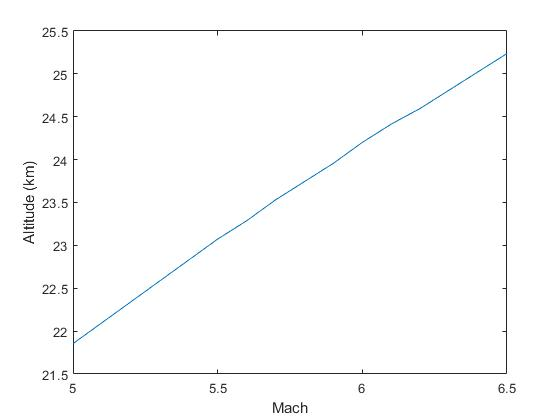
\includegraphics[width=0.6\textwidth]{altVMach}
\caption{Altitude v. Mach}
\label{fig:altVMach}
\end{center}
\end{figure}

\begin{figure}{r}[H]
\begin{center}
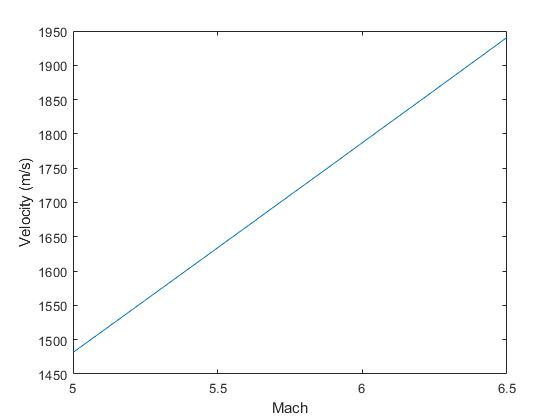
\includegraphics[width=0.6\textwidth]{velVMach}
\caption{Velocity v. Mach}
\label{fig:velVMach}
\end{center}
\end{figure}

\begin{figure}[H]
\begin{center}
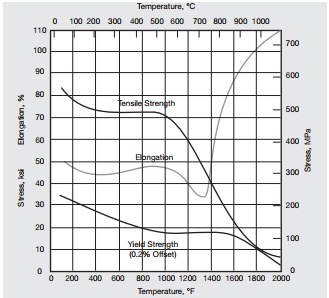
\includegraphics[width=0.6\textwidth]{incoloyPlot}
\caption{Temperature Range Across Combustor Structure \cite{inco}}
\label{fig:incoloyPlot}
\end{center}
\end{figure}

\begin{figure}[H]
\begin{center}
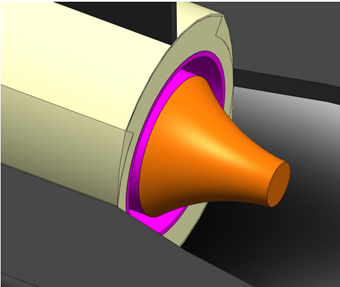
\includegraphics[width=0.5\textwidth]{nozzleIsoView}
\caption{Final Nozzle Design}
\label{fig:nozzleIsoView}
\end{center}
\end{figure}

\begin{figure}[H]
\begin{center}
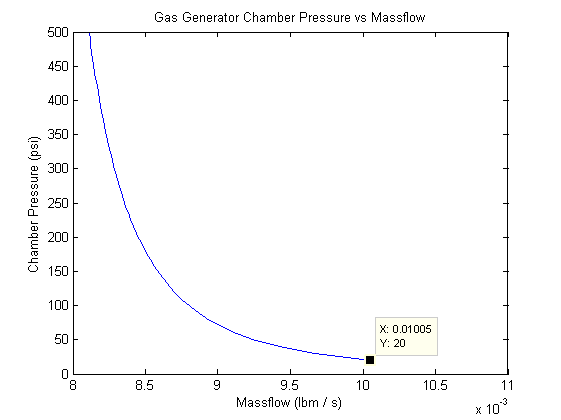
\includegraphics[width=0.6\textwidth]{turboPressureVMdot}
\caption{Turbopump Pressure v. Mass Flow Rate}
\label{fig:turboPressureVMdot}
\end{center}
\end{figure}


\section{Appendix B: Equations}

\begin{equation}
\begin{split}
Re_x=\frac{\rho u x}{\mu}	
If   Re_x<500,000, \text{  Laminar boundary layer} \\
	If   Re_x>500,000, \text{  Turbulent boundary layer}
\end{split}
\label{eqn:reynolds}
\end{equation}


\begin{equation}
Pr=\frac{\mu Cp}{K}
\label{eqn:prandtl}
\end{equation}

\begin{equation}
Nu_x=\frac{h_g x}{K}
\label{eqn:nusselt}
\end{equation}